\documentclass{article}

\usepackage{times}
\usepackage{amssymb, amsmath, amsthm}
\usepackage[margin=1in]{geometry}
\usepackage{graphicx}

\begin{document}

\title{MTH 351 Homework 7}
\author{Philip Warton}
\date{\today}
\maketitle
\section*{1}
Let $f(x) = \dfrac{1}{x+1}$. Points are evenly spaced such that $0 = x_1 < x_2 < \dots < x_n = 2$. We can begin by taking the $n$th derivative of $f$.
\begin{align*}
f(x) & = (x+1)^{-1} \\
f'(x) & = (-1)(x+1)^{-2} \\
f''(x) & = (-1)(-2)(x+1)^{-3} \\
&\vdots \\
f^n(x) & = (-1)^nn!(x+1)^{-n-1}
\end{align*}
We write 
\[ |f(x) - P_n(x)| \leqslant \dfrac{1}{n} \left(\dfrac{b-a}{n-1}\right)^n max_{[a,b]}|f^n(x)| \]
This is equivalent to 
\[ |f(x) - P_n(x)| \leqslant \dfrac{1}{n} \left(\dfrac{2}{n-1}\right)^nmax_{[0,2]}\dfrac{n!}{|(x+1)^{n+1}|} \]
This number is largest when $x = 0$, so we have
\[|f(x) - P_n(x)| \leqslant \dfrac{1}{n} \left(\dfrac{2}{n-1}\right)^nn! \]
To guarentee this quantity to be lower than $10^{-4}$ we must have $n \geqslant 31$.

\section*{2}
See Matlab code turned in on canvas. Some plots are shown here, but not all.
\begin{figure}
\caption{$P_n$ on the First Function}
\centering
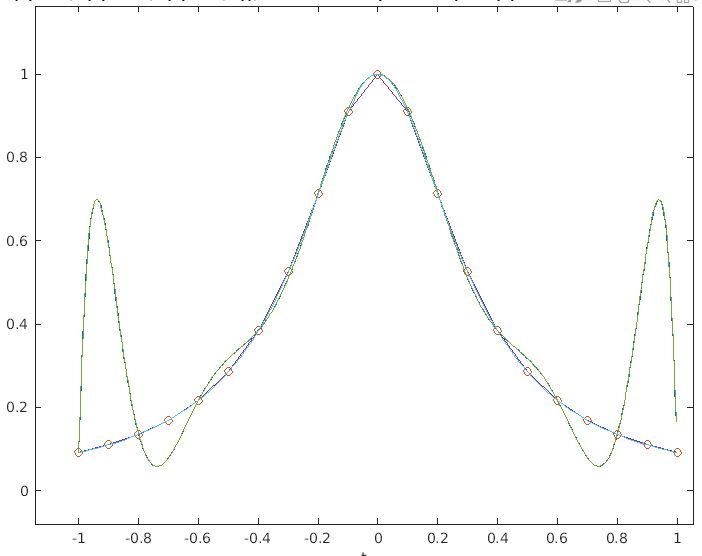
\includegraphics[scale=.4]{hw_7_plot_g1}
\end{figure}

\begin{figure}
\caption{$Q_n$ on the First Function}
\centering
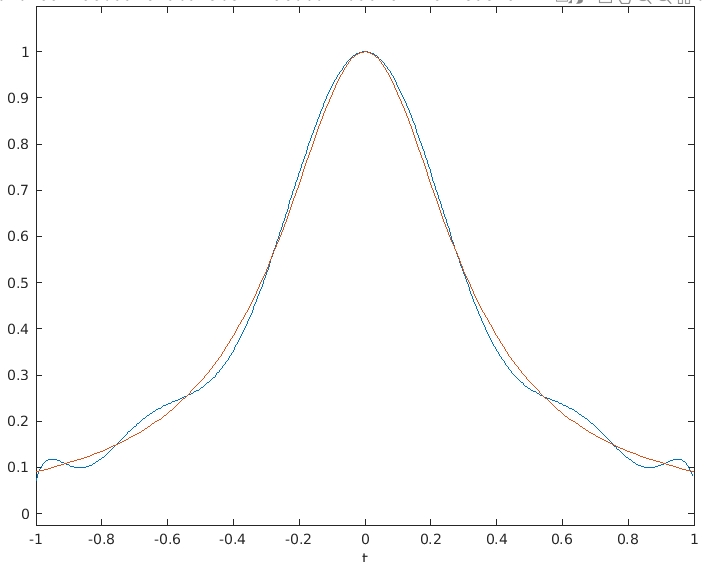
\includegraphics[scale=.4]{hw_7_plot_g2}
\end{figure}

\begin{figure}
\caption{$P_n$ on the Second Function}
\centering
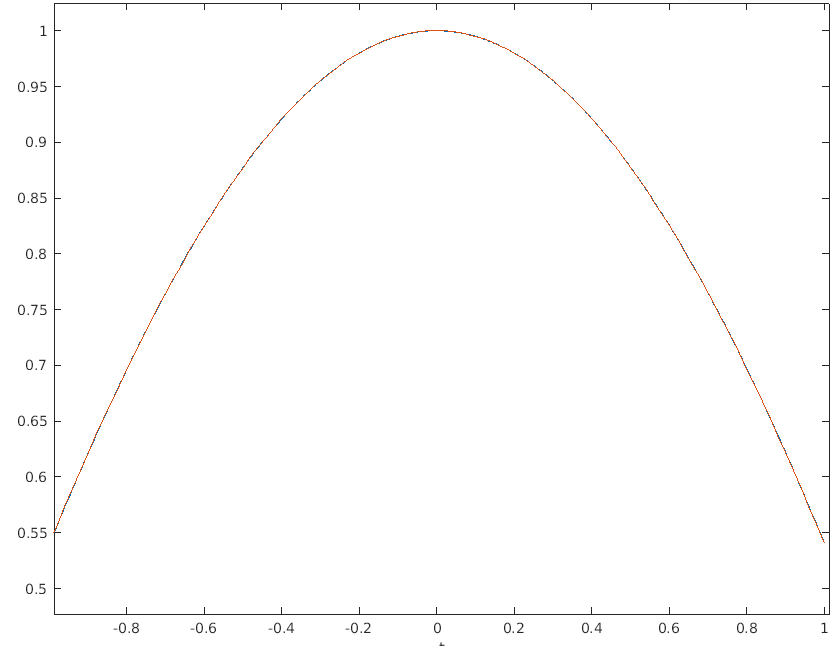
\includegraphics[scale=.4]{hw_7_plot_f1}
\end{figure}

\begin{figure}
\caption{$Q_n$ on the Second Function}
\centering
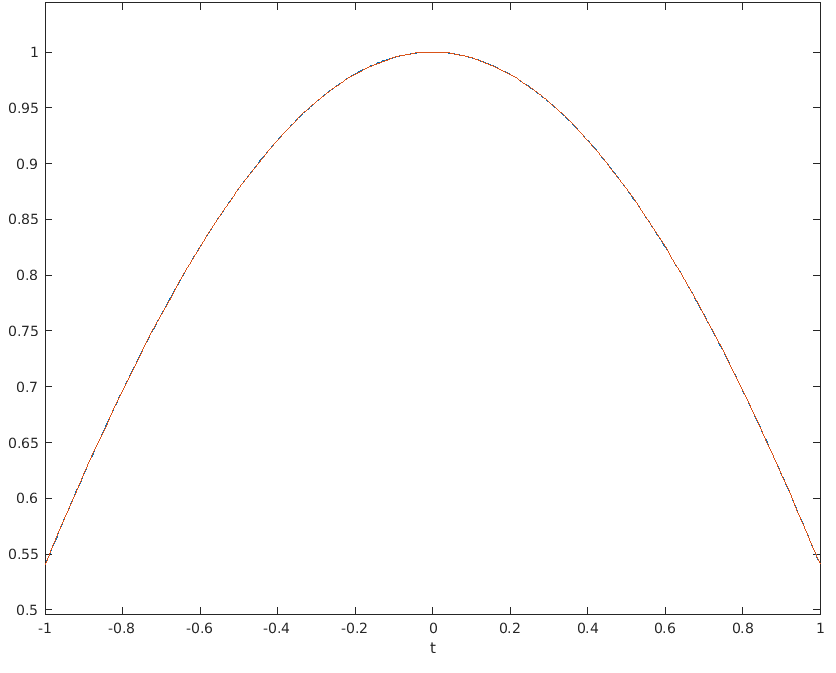
\includegraphics[scale=.4]{hw_7_plot_f2}
\end{figure}


Shown here are the two different graphs, one for $P_n$ and one for $Q_n$. It appears that $Q_n$ better approximates the function, with unevenly spaced points closer to the bounds $a$ and $b$. I speculate that this is because the polynomial behavior is more extreme towards the end points, and this can be mitigated by having more data near said end points.

For the cosine function, both approximations look pretty spot on, so it becomes difficult to say that one is better than the other in this case.

\section*{3}
\subsection*{(a)}
For a given $j$, we write 
\[s_j (x_j) = \frac{M_j - M_{j+1}}{2(x_j-x_{j+1})}(x^2-x_j^2) + \frac{x_jM_{j+1}-x_{j+1}M_j}{x_j-x_{j+1}}(x-x_j) + y_j \]
\subsection*{(b)}
For the equation to hold, we must have that
\[(M_j + M_{j+1})\frac{x_{j+1}-x_j}{2} = y_{j+1}-y_j\]
\subsection*{(c)}
Using Matlab, we get
$\\ M_1 = 0, \\ M_2 = 0.4423, \\M_3 = 0.3803, \\M_4 = 1.2919, \\M_5 = 2.0048, \\M_6 = 0.8524, \\M_7 = -3.7095, \\M_8 = 0.4128, \\M_9 =- 2.0851, \\M_{10} = 1.2625, \\M_{11} = -1.7048 $

\begin{figure}
\caption{Quadratic Spline on the First Function}
\centering
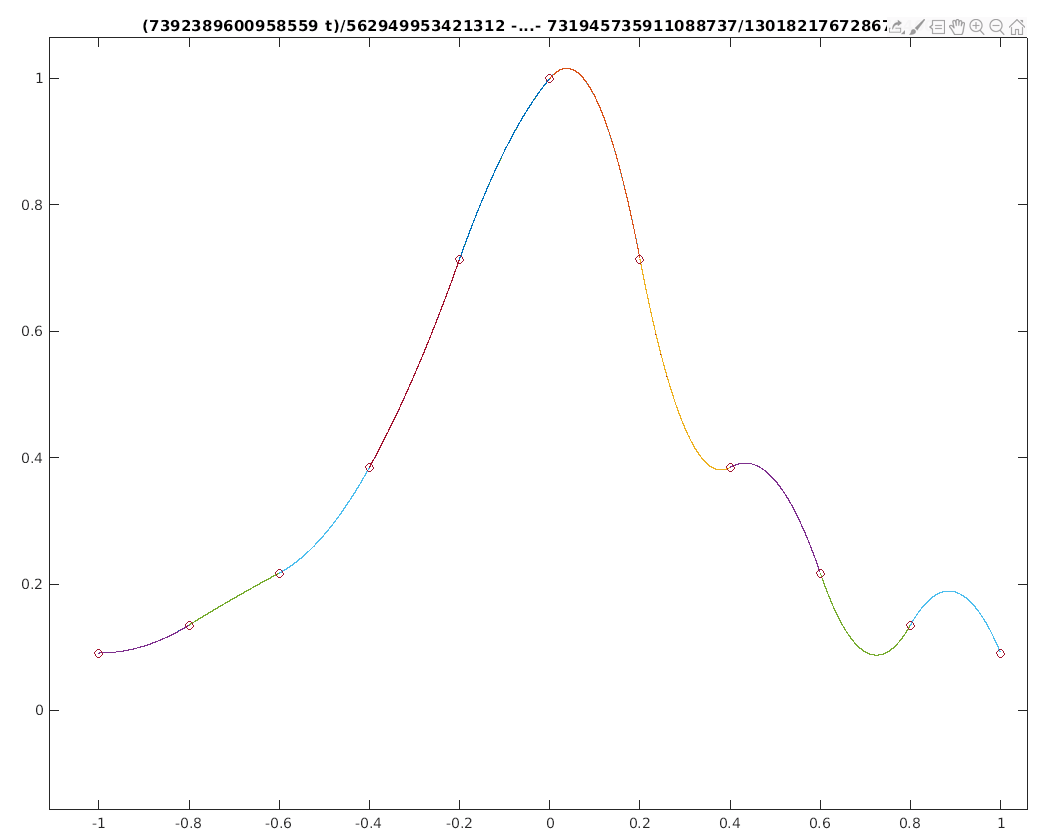
\includegraphics[scale=.4]{hw_7_plot_p3}
\end{figure}
\end{document}